\documentclass{standalone}
\usepackage{tikz}
\usepackage{ctex,siunitx,ninecolors}
\setCJKmainfont{Noto Serif CJK SC}
\usepackage{tkz-euclide}
\usepackage{amsmath}
\usetikzlibrary{patterns, calc}
\usetikzlibrary {decorations.pathmorphing, decorations.pathreplacing, decorations.shapes}
\newcommand{\posthead}[2][gray]{
  \begin{scope}[#2]
    \fill[left color=#1,right color= #1,middle color=#1!20](0,0)ellipse(0.05 and 0.02);
    \fill[left color=#1,right color= #1,middle color=#1!20](0.05,0)rectangle(-0.05,0.07);
    \fill[left color=#1,right color= #1,middle color=#1!20](-0.06,0.07)arc(-180:0:0.06 and 0.02)--(0.06,0.15)--(0.05,0.16)--(-0.05,0.16)--(-0.06,0.15)--cycle;
    \fill[#1!50!gray](0,0.16)ellipse(0.05 and 0.02);
    \foreach \x in {75,45,15,-15,-45,-75}
    {
      \draw[very thin,#1!50!gray]({0.05*sin(\x)},{0.16-0.02*cos(\x)})--({0.06*sin(\x)},{0.15-0.02*cos(\x)})--++(0,-0.08);
    }
  \end{scope}
}
\begin{document}
\small
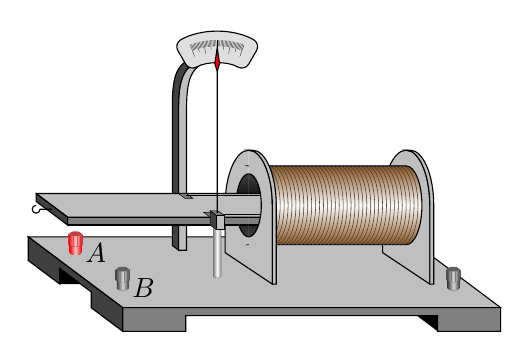
\begin{tikzpicture}[>=latex,scale=1.0]
  \fill(-2.4,-1)rectangle++(1,0.2)(2.4,-1.6)--++(-0.4,0.3)--++(0,0.2)--++(0.4,-0.3);
  \draw[fill=lightgray](-2.8,-0.4)--++(4.8,0)--++(1.2,-0.9)--++(-4.8,0)--cycle;
  \draw[fill=darkgray](-2.8,-0.4)--++(1.2,-0.9)--++(0,-0.3)--++(-0.4,0.3)--++(0,0.2)--++(-0.4,0.3)--++(0,-0.2)--++(-0.4,0.3)--cycle;
  \draw[fill=gray](-1.6,-1.3)--++(4.8,0)--++(0,-0.3)--++(-0.8,0)--++(0,0.2)--++(-3.2,0)--++(0,-0.2)--++(-0.8,0)--cycle;
  \draw[fill=darkgray](-0.411,1.892)..controls(-0.773,1.792)and(-0.890,1.763)..(-0.89,1.2)--(-0.89,-0.57)--(-0.97,-0.51)--(-0.97,1.26)..controls(-0.970,1.809)and(-0.853,1.837)..(-0.491,1.938);
  \draw[fill=lightgray](-0.311,1.892)..controls(-0.673,1.792)and(-0.790,1.763)..(-0.79,1.2)--(-0.79,-0.57)--(-0.89,-0.57)--(-0.89,1.2)..controls(-0.890,1.763)and(-0.773,1.792)..(-0.411,1.892);
  \draw[fill=lightgray](0,-0.8)--(-0.3,-0.6)--(-0.3,0)arc(180:90:0.3 and 0.7);
  \fill[top color=darkgray,bottom color=darkgray,middle color=black,draw=black](0,0)ellipse(0.16 and 0.4);
  \draw[fill=lightgray,line join=round](-2.7,0.15)--(1.2,0.15)--(1.8,-0.15)--(-2.3,-0.15)--cycle;
  \draw[fill=gray](1.8,-0.15)rectangle(-2.3,-0.25);
  \draw[fill=darkgray](-2.7,0.15)--(-2.3,-0.15)--(-2.3,-0.25)--(-2.7,0.05)--cycle;
  \draw[fill=gray,very thin](-0.89,0.15)--(-0.79,0.15)--(-0.71,0.09)--(-0.81,0.09)--cycle;
  \draw[fill=gray,very thin](-0.49,-0.15)--(-0.39,-0.15)--(-0.47,-0.09)--(-0.57,-0.09)--cycle;
  \draw(-0.8,0.12)--(1,0.12);
  \draw(-0.48,-0.12)--(1,-0.12);
  \fill[left color=gray,right color=gray,middle color=white](-0.45,-0.9)arc(180:360:0.05 and 0.02)--++(0,0.6)--++(-0.1,0)--cycle;
  \draw[fill=gray,very thin](-0.49,-0.07)--(-0.39,-0.07)--(-0.31,-0.13)--(-0.41,-0.13)--cycle;
  \draw[fill=darkgray,very thin](-0.49,-0.07)--(-0.41,-0.13)--(-0.41,-0.31)--(-0.49,-0.25)--cycle;
  \draw[fill=lightgray,very thin](-0.31,-0.13)rectangle(-0.41,-0.31);
  \draw[fill=lightgray](1.7,-0.6)--(1.7,0)arc(180:0:0.3 and 0.7)--(2.3,-1.0)--cycle;
  \fill[top color=brown4,bottom color=brown4,middle color=brown9!10,draw=black](0,-0.5)arc(-90:90:0.2 and 0.5)--(2,0.5)arc(90:-90: 0.2 and 0.5)--cycle;
  \foreach \x in {0.05,0.1,...,1.98} { \draw[very thin,darkgray] (\x,-0.5)arc(-90:90:0.2 and 0.5);}
  \draw[fill=lightgray,even odd rule](0,0.7)arc(90:0:0.3 and 0.7)--(0.3,-1.0)--(0,-0.8)(0,0.4)arc(90:-90:0.16 and 0.4);
  \draw[fill=lightgray](2.3,-1.0)--++(0.05,0)--++(0,1)arc(0:90:0.3 and 0.7)--++(-0.05,0)arc(90:0:0.3 and 0.7)--cycle;
  \draw[fill=lightgray](0.3,-1.0)--++(0.05,0)--++(0,1)arc(0:90:0.3 and 0.7)--++(-0.05,0)arc(90:0:0.3 and 0.7)--cycle;
  \draw[thin](-2.5,-0.05)--(-2.65,-0.05)arc(360:90:0.05);
  \draw[rounded corners=1mm,fill=lightgray!50]([shift=(120:0.7)]-0.4,1.1)arc(120:60:0.7)--++(60:0.4)arc(60:120:1.1)--cycle;
  \foreach \x in {110,100,90,80}
  {
    \draw[ultra thin]([shift=(\x:1.0)]-0.4,1.1)--++(\x:-0.16);
    \draw[ultra thin]([shift=(\x-5:1.0)]-0.4,1.1)--++(\x-5:-0.12);
    \foreach \y in {1,2,3,4,6,7,8,9}
    {
      \draw[ultra thin]([shift=(\x-\y:1.0)]-0.4,1.1)--++(\x-\y:-0.08);
    }
  }
  \draw[ultra thin]([shift=(70:1.0)]-0.4,1.1)--++(70:-0.16);
  \draw[fill=red](-0.4,-0.1)--++(0,1.8)--++(-0.03,0.1)--++(0.03,0.2)--++(0.03,-0.2)--++(-0.03,-0.1);
  \posthead[red]{yshift=-0.6cm,xshift=-2.2cm,scale=1.5}
  \posthead[darkgray]{yshift=-1.05cm,xshift=-1.6cm,scale=1.5}
  \posthead[darkgray]{yshift=-1.05cm,xshift=2.6cm,scale=1.5}
  \node at (-2.2,-0.6)[right]{$A$};
  \node at (-1.6,-1.05)[right]{$B$};
\end{tikzpicture}
\end{document}